\chapter{Introduction}\label{ch:Introduction}
\todo{problem statement: As the IoT market is still in its infancy a main communication protocol should be chosen based on several performance metrics, which allows companies to compete on equal terms.}


\section{Motivation}
%Why is the topic of interest? 
%New technology
%	IoT development
%	Massive number of devices
%	5G

\section{Problem Analysis}
%What are the problem?
%	Many standards 
%	Not really tested
%	Nothing really deployed
%	Unity
%Why do we have the problem?
%	New technology
%	Money
%	Competiveness
%Problem statement!

\section{Solution Analysis}
%What have been done before?
%	Last thesis
%	Some test into battery lifetime
%	Theoretic calculations
%What could be a solution for the problem?
%	An IoT emulator
%	Comparison of theoretic metrics
%	Choose blindly
%	Deploy a test case
%What are we working with and why?
%	An IoT emulator
%	Massiveness
%	Power
%Why not reliability


%\textbf{Motivation}
The market of cellular technologies is changing and the need for a new type of technology has arisen. This is the need for \gls{LPWA} networks, \gls{LPWA} networks are classified by three main aspects: long battery lifetime, low cost units and huge amount of users. With the development of \gls{LPWA} networks, especially in regards to the evolution of 5G as well as \gls{IoT} technologies increasing amount of focus, has come to the massive part of communication. It was estimated that in 2016 0.4 billion devices were of the \gls{LPWA} type, but this is predicted to reach 1.5 billion by 2021, equivalent to a yearly growth rate of 27 \% \citep{mobi-report}. This change sets some requirements that is not achievable with existing systems, however to accommodate this several technologies have been developed.


Generally the new technologies are classified into categories: (i) cellular networks based solution (ii) proprietary solutions as can be seen in \autoref{fig:IoT_protocol_overview}. All these technologies are competing to be the main standard of massive \gls{IoT} communication. 
%\textbf{Objective}

\begin{figure}[H]
\centering
%\resizebox{\textwidth}{!}{
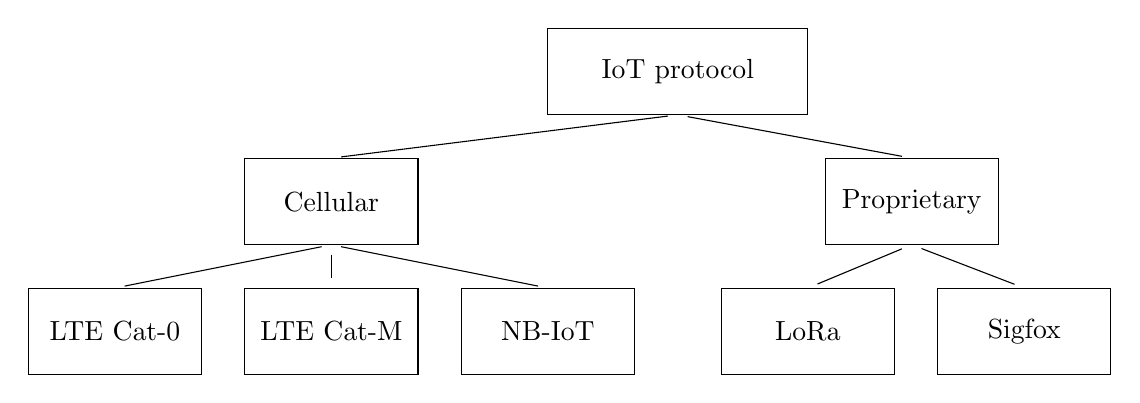
\begin{tikzpicture}[scale=0.11]
\draw  (10,100) rectangle (40,90);
\node at (25,95) {IoT protocol};
\draw  (-25,85) rectangle (-5,75);
\node at (-15,80) {Cellular};
\draw  (42,85) rectangle (62,75);
\node at (52,80) {Proprietary};

\draw  (-50,70) rectangle (-30,60);
\node at (-40,65) {LTE Cat-0};
\draw  (-25,70) rectangle (-5,60);
\node at (-15,65) {LTE Cat-M};
\draw  (0,70) rectangle (20,60);
\node at (10,65) {NB-IoT};
\draw  (30,70) rectangle (50,60);
\node at (40,65) {LoRa};
\draw  (55,70) rectangle (75,60);
\node at (65,65) {Sigfox};


%\draw  (-2,47) ellipse (4 and 4);
%\draw (-2,51) -- (48,51) -- (48,43) -- (-2,43);
%\node at (-2,47) {A};
%\node [anchor=west] at (8,47) {Reliability};
%
%\draw  (-2,35) ellipse (4 and 4);
%\draw (-2,39) -- (48,39) -- (48,31) -- (-2,31);
%\node at (-2,35) {B};
%\node [anchor=west] at (8,35) {Energy consumption};
%
%\draw  (-2,23) ellipse (4 and 4);
%\draw (-2,27) -- (48,27) -- (48,19) -- (-2,19);
%\node at (-2,23) {C};
%\node [anchor=west] at (8,23) {Massiveness};

\node (v1) at (25,90) {};
\node (v2) at (-15,85) {};
\node (v3) at (52,85) {};
\node (v4) at (-15,75) {};
\node (v5) at (-40,70) {};
\node (v6) at (-15,70) {};
\node (v7) at (10,70) {};
\node (v8) at (52,75) {};
\node (v9) at (40,70) {};
\node (v10) at (65,70) {};
\draw  (v1) edge (v2);
\draw  (v1) edge (v3);
\draw  (v4) edge (v5);
\draw  (v4) edge (v6);
\draw  (v4) edge (v7);
\draw  (v8) edge (v9);
\draw  (v8) edge (v10);
\end{tikzpicture}%}
\caption{\gls{IoT} protocol overview}
\label{fig:IoT_protocol_overview}
\end{figure}


Even though, the technologies in question have already been designed most is still in their infancy, because of this most metrics that can be found for the different protocols, are to our knowledge based on a theoretic approach and not on actual measurements. 

\begin{table}[H]
\centering
\resizebox{\textwidth}{!}{%
\begin{tabular}{|l|l|l|l|l|l|}
\hline
\textbf{Feature}            & \textbf{LoRa}           & \textbf{Sigfox}        	   & \textbf{LTE Cat-1} & \textbf{LTE-M}    & \textbf{NB-IoT} \\ \hline
Modulation                  & SS Chirp                   & UNB/GSK/BPSK                & OFDMA              & OFDMA                 & OFDMA           \\ \hline
Rx bandwidth                & 500-125 kHz                & 100 Hz                      & 20 MHz             & 20-1.4 MHz            & 200 KHz         \\ \hline
Data Rate                   & 290 bps – 50 Kbps          & 100 bps / 8 bytes max 	   & 10 Mbps       		& 200 kbps – 1 Mbps     & 20 Kbps         \\ \hline
Max output power            & 20 dBm                     & 20 dBm                      & 23 – 46 dBm        & 23/30 dBm             & 20 dBm          \\ \hline
\begin{tabular}[c]{@{}l@{}}Battery lifetime \\ (2000 mAh)\end{tabular}& 105 months ($\sim$9 years) & 90 months (7.5 years)  &   & 18 months (1.5 years) &   \\ \hline
Link budget                 & 154 dB                     & 151 dB                      & 130 dB+            & 146 dB                & 150 dB          \\ \hline
Security                    & Yes                        & No                          & Yes                & Yes                   &                 \\ \hline
\end{tabular}%
}
\caption{Comparison of performance metrics between cellular solutions and proprietary solutions \citep{NB_comp}}%http://www.3glteinfo.com/lora/lora-advantages/}
\label{tab:tech_comparison1}
\end{table}



% Please add the following required packages to your document preamble:
% \usepackage{graphicx}
%\begin{table}[H]
%\centering
%%\resizebox{\textwidth}{!}{%
%\begin{tabular}{|l|l|l|l|l|}
%\hline
%\textbf{Feature}   & \textbf{\begin{tabular}[c]{@{}l@{}}Release 8\\ Cat 4\end{tabular}} & \textbf{\begin{tabular}[c]{@{}l@{}}Release 8\\ Cat 1\end{tabular}} & \textbf{\begin{tabular}[c]{@{}l@{}}Release 13\\ LTE-M\end{tabular}} & \textbf{\begin{tabular}[c]{@{}l@{}}Release 13\\ NB-IoT\end{tabular}} \\ \hline
%Downlink speed     & 150 Mbps                                                           & 10 Mbps                                                            & 384 kbps - 1Mbps                                                    & 170-250 kbps                                                         \\ \hline
%Uplink speed       & 50 Mbps                                                            & 5 Mbps                                                             & 384 kbps - 1Mbps                                                    & 50-144 kbps                                                          \\ \hline
%Number of antennas & 2                                                                  & 2                                                                  & 1                                                                   & 1                                                                    \\ \hline
%Duplex mode        & Full duplex                                                        & Full duplex                                                        & Full or Half duplex                                                 & Half duplex                                                          \\ \hline
%Receive bandwidth  & 20 MHz                                                             & 20 MHz                                                             & 1.4 MHz                                                             & 200 kHz                                                              \\ \hline
%Transmit power     & 23 dBm                                                             & 23 dBm                                                             & 20 dBm                                                              & 23 dBm                                                               \\ \hline
%Modem complexity   & 100 \%                                                             & 80 \%                                                              & 20 \%                                                               & \textless15 \%                                                       \\ \hline
%Voice              & Yes                                                                & Yes*                                                               & Yes                                                                 & No                                                                   \\ \hline
%Mobility           & Full                                                               & Full                                                               & Limited                                                             & \begin{tabular}[c]{@{}l@{}}Fixed-Idle\\ Mode Only\end{tabular}       \\ \hline
%\end{tabular}%
%%}
%\caption{Comparison of cellular solutions \citep{CAT_comp}} %https://www.digi.com/blog/cellular/introduction-to-lte-m-cellular-technology/
%\label{tab:tech_comparison2}
%\end{table}

It can be seen from \autoref{tab:tech_comparison1}, that the different technologies have different advantages. The main differences between them are the bandwidth of the receiver as well as the battery lifetime. 

As none of the protocols have been deployed at a large scale, it brings up different concerns especially because the massiveness in question is several magnitudes larger than anything seen before. Therefore to choose the main standard a lot of metrics are taken into consideration divided into three domains: reliability, energy consumption and massiveness i.e. the amount of supported users per km$^2$ or cell. One of the aims of \gls{IoT} devices is a battery lifetime of around 10 years, to achieve this requirement for the energy consumption is of course a key metric. With the scope of billions of devices, several metrics in regards to the massiveness will also be extremely important. Because of the long lifetime coupled with the extreme number of devices the reliability also needs to be very high as it is not feasible to replace devices quickly. \todo{Either add payload as a extra domain or rewrite the part about reliability}

This leads to the problem statement:
\begin{center}
\textbf{As the IoT market is still in its infancy the proposed protocols needs to be evaluated based on metrics of the reliability, energy consumption and massiveness to choose a main IoT protocol.}
\end{center}
%\todo{This statement focus on us chosen the right protocol

%Several different metrics can be tested for each of the domains some are protocol specific others while others are more general. Examples of performance metrics are:
%
%\begin{itemize}
%	\item[\textbf{A}] \textbf{Massiveness}
%	\begin{itemize}
%		\item Time to connect vs. connection request per second 
%		\item Data rate vs. number of users
%		\item Spectrum use vs. number of users
%		\item Interference level vs. number of users
%	\end{itemize}		
%	\item[\textbf{B}] \textbf{Energy consumption}
%	\begin{itemize}
%		\item Energy consumption vs. data rate
%		\item Energy consumption vs. coverage level
%		\item Energy consumption vs. operation mode
%		\item Energy consumption vs. number of UEs
%		\item Energy consumption vs. cellular protocol
%		\item Energy consumption cellular vs. proprietary
%	\end{itemize}
%	\item[\textbf{C}] \textbf{Reliability}
%	\begin{itemize}
%		\item Delay
%		\item \gls{BER} vs. \gls{SINR}/\gls{MCL} vs. protocol
%	\end{itemize}
%\end{itemize}

The focus of the project is to design an emulator combining both software and hardware, that can test how the standards perform in these domains. For this purpose emulation of multiple low performance \gls{IoT} devices is needed. The system should also be able to simulate neighbouring cells to achieve realistic channel conditions. Implementation of a signal processing method that allow to change to different channel models would be optimal. The aim being a customizable emulator which provide performance metrics of the different protocol designs.

%\textbf{Limits of project} \todo{check this when it is decided to to do track 1 or 2}\\
However as this is a huge endeavour, the focus will be on the core principles of this making a proof of concept emulator. When making an emulator it generally only works for a single protocol so designing it for several protocols would be very time consuming and it is chosen that the benefit of supporting several protocols is not worth the extra time it takes to design the emulator. Another factor is the project will build upon existing software as just designing the \gls{BSE} or \gls{IoT} device emulator could easily be an entire project in itself. Based on this different factors are taken in to account when choosing the protocol for the project which can be seen in \autoref{tab:protocol_decision}.

\begin{table}[H]
\centering
\resizebox{\textwidth}{!}{
\begin{tabular}{|c|c|c|c|c|c|} \hline
					& \textbf{LTE Cat-0}& \textbf{LTE Cat-M}	& \textbf{NB-IoT}	& \textbf{LoRa}	& \textbf{Sigfox}	\\ \hline
Licensed spectrum	& Yes				& Yes					& Yes				& No			& No				\\ \hline
\gls{BS} emulator	&  Amarisoft &  Amarisoft & {\begin{tabular}{c}  Amarisoft \\ * SRS \end{tabular}} & \begin{tabular}{c}  The Things Industries \\ * LoRa Server \end{tabular} &   \\ \hline

\gls{UE} emulator	&  & {\begin{tabular}{c}  Amarisoft \\ Asiatelco \\ AT\&T \\ Digi \\ Fibocom \\ Gemalto \\ H3C \\ Huawei \\ LinkLabs \\ Longsung \\ Meig \\ Mobiletek \\ Multitech \\ Neoway \\ NimbeLink \\ pycom \\ Quectel \\ Sierra Wireless \\ SimCom \\ Skyworks \\ Telit \\ u-blox \\ ZTEWelink  \end{tabular}} & {\begin{tabular}{c}  Amarisoft \\ Cheerzing \\ CMCC \\ Digi \\ H3C \\ Lierda \\ Longsung \\ Meig \\ Mobiletek \\ Mokuai \\ Neoway \\ pycom \\ Quectel \\ Sierra Wireless \\ SimCom \\ Skyworks \\ Telit \\ u-blox \\ ZTEWelink \\ * SRS \end{tabular}} & {\begin{tabular}{c}  The Things Industries \\  Miromico \\  Telit \end{tabular}} &	{\begin{tabular}{c}   Murata \\  Telit \\ * Telefonicaid \end{tabular}} \\ \hline
Modem complexity	& High 				& Middle 				& Middle 			& Middle 		& Low				\\ \hline
\end{tabular}}
\raggedright \scriptsize{ * Open source solutions} 
\caption{Commercial solutions available for the different protocols. \citep{UE_list, Amarisoft_solutions, SRS_solutions, LORA_solutions, Things_solutions, Mira_solutions, Telit_solutions, telefonicaid_solutions, murata_solutions}}%The solutions presented is found from google searches and might not show a complete image of available solutions.}
\label{tab:protocol_decision}
\end{table}

%Based on \autoref{tab:protocol_decision} the \gls{NB-IoT} protocol is chosen. This is based on the fact it uses the licensed spectrum as well as the solutions available. Also it is chosen to primarily look at the massiveness aspect of the protocol. \todo{check with germans comments}%check this again before hand-in}

When looking at \autoref{tab:protocol_decision} it can be seen that for \gls{LTE} Cat-0 no \gls{UE} emulator was found for this protocol. This has to do with the development of \gls{LTE} Cat-M and \gls{NB-IoT} which shares most of the same properties but are more specialised to the \gls{IoT} market. It can also be seen that for both \gls{LTE} Cat-M and \gls{NB-IoT} multiple \gls{UE} emulators exist, this has to do with both protocols being cellular protocols developed by \gls{3GPP} this is very desired by the industry for various reasons. For \gls{LoRa} there exists both  \gls{BS} and \gls{UE} emulators, it is also one of the most used proprietary protocols on the market. For the Sigfox protocol no \gls{BS} emulators has been found. Based on these investigations it is chosen to use the \gls{NB-IoT}, both because it has a lot of emulators already but mainly because it has an open source \gls{UE} emulator \todo{Are the NB-IoT UE open source, did we not get it through Keysight?}. This is desired as to allow for modifications of the \gls{UE} software.  


To make the most realistic emulation the final solution needs to work in real time, this sets some limitations performance wise. One of the problems associated with real time computation is the computational capacity meaning the emulator will not be able to handle several thousands \gls{UE}s simultaneously as the deployed system is required to. This is further explored in \todo{make ref to appropriate chapter}.

As all of these protocols are new the main focus will be on setting up a proof of concept model, this means that only a single cell will be emulated furthermore the emulator will only use a single channel model.\todo{Need more fill, as why we do not focus on these parts and also very hard cut off for a section}





%To make an emulator for all the technologies mentioned would not be feasible in the time frame of the project therefore one is picked to prove the concept. The \gls{NB-IoT} is chosen because it provides a good compromise of data rate and battery life time, as well as being compatible with \gls{LTE}. Another factor for choosing \gls{NB-IoT} is that Keysight has provided the opportunity to test the system with their UXM base station, as well as \gls{SRS} developing an \gls{UE} for the \gls{NB-IoT} system. 

 
%To achieve this existing software will form the base but might need to be redesigned to minimize duplicate operations along with fulfilling the massive aspect. Finally 

%	\begin{itemize}
%		\item only a few devices
%		\item only a single channel model
%		\item no interfering neighbours
%		\item probably no API
%	\end{itemize}

%\newpage
%\begin{itemize}
%	\item Objective	(NB emulator)
%	\begin{itemize}
%		\item scalable embedded hardware/software combination
%		\item multiple/massive low performance IoT devices 
%		\item Re-design of an NB-IoT software modem that minimizes the duplicated operations
%		\item Implementation of a signal processing method that allows the generation of a waveform containing multiple transmitting devices geographically distributed, having different channel characteristics. (Optional)
%		\item how the network will perform under massive traffic and (ii) how the interferences of neighboring cells will impact the overall performance
%	\end{itemize}
%	\item Motivation
%	\begin{itemize}
%		\item Up and coming technology
%		\item alternative cellular network
%		\item problem of massiveness
%	\end{itemize}
%	\item Technologies
%	\begin{itemize}
%		 \item LTE-M
%		 \item CAT 1
%		 \item CAT 0
%		 \item CAT M1
%		 \item CAT NB1
%		 \item Sigfox
%		 \item LoRa
%	\end{itemize}
%	\item Limits of project
%	\begin{itemize}
%		\item only a few devices
%		\item only a single channel model
%		\item no interfering neighbours
%		\item probably no API
%	\end{itemize}
%\end{itemize}

